\begin{frame}{Subdomain Interfaces and Energy Minimization}
    \begin{columns}
    \begin{column}{0.5\textwidth}
      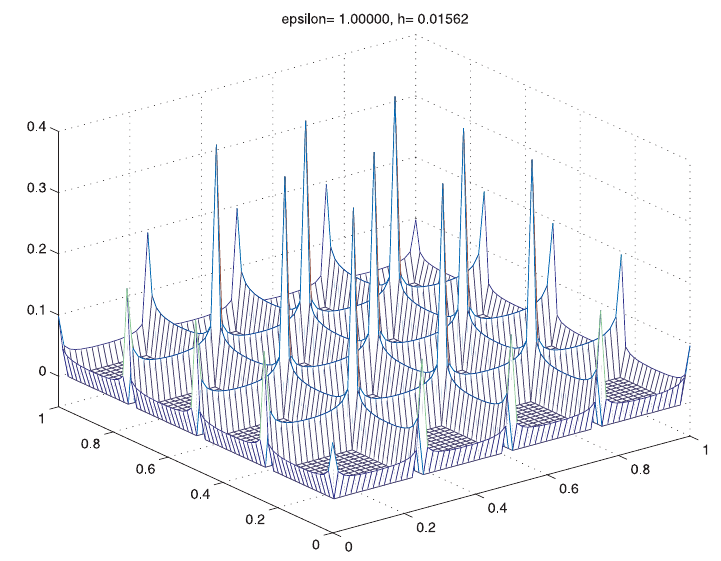
\includegraphics[width=\textwidth]{figures/MG/XuZikatanovLambda} \\
      {\small [Xu and Zikatanov 2004]}
    \end{column}
    \begin{column}{0.5\textwidth}
      \begin{itemize}
      \item minimize energy of all basis functions (columns of $P$) subject to
        \begin{itemize}
        \item fixed compact support
        \item partition of unity (near-null space)
        \end{itemize}
      \item enforce partition of unity using Lagrange multipliers
        \begin{itemize}
        \item $\lambda(x) = 0$ in coarse element interiors
        \item means that globally optimal coarse basis functions are harmonic extensions of \emph{some} interface values
        \end{itemize}
      \end{itemize}
    \end{column}
  \end{columns}
\end{frame}

\begin{frame}{Local edge/face-centered problems}
  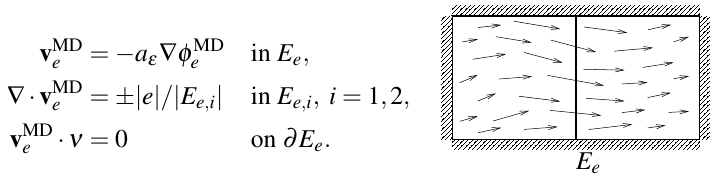
\includegraphics[width=0.9\textwidth]{figures/MG/ArbogastMultiscaleDual}
  \begin{itemize}
  \item Arbogast's multiscale dual-support elements for porous media
    \begin{itemize}
    \item inconsistent for unaligned anisotropy
    \item homogenization approach: upscale effective conductivity tensor from solution of periodic dual-support problem
    \end{itemize}
  \item Dohrmann and Pechstein's balancing domain decomposition for elasticity with unaligned coefficients
    \begin{itemize}
    \item balance ``torn'' interface values $u_{ie},u_{je}$, written in terms of subdomain Schur complements
    \item $\bar f_e = S_{iee} u_{ie} + S_{jee} u_{je}$: sum of forces required along face $e$ to displace subdomains $i$ and $j$ by $u_{ie}, u_{je}$
    \item $\bar u_e = (S_{iee} + S_{jee})^{-1} \bar f_e$: continuous displacement
    \item equivalent to a (different) dual-support basis
    \end{itemize}
  \end{itemize}
\end{frame}
